\documentclass[10pt, a4paper]{article}

\usepackage[english]{babel}
\usepackage[margin=2cm, nohead]{geometry}
\usepackage{parskip}
\usepackage{listings}
\usepackage{array}
\usepackage{arydshln}
\usepackage[T1]{fontenc}
\usepackage{amsmath}
\usepackage{graphicx}
\usepackage{tikz}
\usetikzlibrary{shapes,decorations.pathreplacing,positioning,calc,fit}
%\usetikzlibrary{shapes.multipart}


\begin{document}

\begin{center}
\LARGE Block Heap Layout
\end{center}

\section{Abstract}

In this document I will present an alternative memory layout for binary heaps called block heap layout (BHL).
In a $d$-BHL subtrees of height $d$ are stored continuously opposed to the standard layout for binary trees which stores nodes layer by layer.
I will first define the BHL structure and then analyse it in comparison to the standard binary tree layout.

\section{Definition}

The following illustration represents one block in the $d$-BHL structure (the number in the node refers to its position when saved in the array).

\begin{tikzpicture}[level/.style={sibling distance=3cm/#1,level distance=1cm}]
\node [rectangle,draw] (n0){0}
	child {node [rectangle,draw] (n1) {1}
		child {node{$\vdots$}
			child {node [rectangle,draw,left] (n3) {$2^d-1$}}
		}
		child {node{$\vdots$}}
	}
	child {node [rectangle,draw] (n2) {2}
		child {node{$\vdots$}}
		child {node{$\vdots$}
			child {node [rectangle,draw,right] (n4) {$2^{d+1}-2$}}
		}
	};
    
\path (n3) -- (n4) node [midway] {$\cdots$};

\coordinate (cd1) at ($(n4)+(1.5,0)$);
\draw[<->,] 
(cd1) -- (cd1|-n0.east) node [midway,fill=white] {$d$};
\end{tikzpicture}

Let $D=2^{d+1}$. In order to use the BHL structure for heaps of any size, we can make each of the $D$ children of leafs in a block root nodes of another block.
Thus a $D$-ary tree is formed by the blocks.

\begin{tikzpicture}[
	level/.style={sibling distance=3cm/#1,level distance=1cm},
	child anchor=north,parent anchor=south,
	every text node part/.style={align=center},
	nd/.style={isosceles triangle,draw,shape border rotate=90, isosceles triangle apex angle=60,inner sep=0,font=\tiny,yshift={-20mm},text width=2cm},
]
\node[nd] {$0\ldots D-2$}
	child{node[nd,left] {$D\ldots 2D-2$}
		child{node[left] {$\vdots$}}
	}
	child{node[nd,left] (a){$2D\ldots 3D-2$}}
	child{node[nd,right] (b){$D^2\ldots D^2+D-2$}};
\path (a) -- (b) node [midway] {$\cdots$};
\end{tikzpicture}

Note that always one index is skipped between two blocks so that the index of each block's root node is divisible by $D$.

Subsequently, an example for a $1$-BHL layout is depicted:

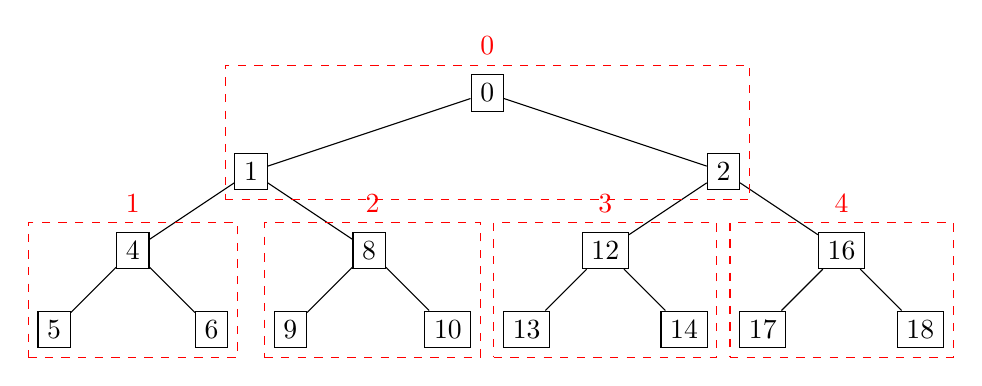
\begin{tikzpicture}[level/.style={sibling distance=6cm/#1,level distance=1cm}]
\node [rectangle,draw] (n0){0}
	child {node[rectangle, draw] (n1) {1}
		child {node[rectangle, draw] (n4) {4}
			child {node [rectangle, draw] (n5) {5}}
			child {node [rectangle, draw] (n6) {6}}
		}
		child {node[rectangle, draw] (n8) {8}
			child {node [rectangle, draw] (n9) {9}}
			child {node [rectangle, draw] (n10) {10}}
		}
	}
	child {node[rectangle, draw] (n2) {2}
		child {node[rectangle, draw] (n12) {12}
			child {node [rectangle, draw] (n13) {13}}
			child {node [rectangle, draw] (n14) {14}}
		}
		child {node[rectangle, draw] (n16) {16}
			child {node [rectangle, draw] (n17) {17}}
			child {node [rectangle, draw] (n18) {18}}
		}
	};
  
\node[draw,red,dashed,fit=(n0) (n1) (n2),label={[red]0}] {};
\node[draw,red,dashed,fit=(n4) (n5) (n6),label={[red]1}] {};
\node[draw,red,dashed,fit=(n8) (n9) (n10),label={[red]2}] {};
\node[draw,red,dashed,fit=(n12) (n13) (n14),label={[red]3}] {};
\node[draw,red,dashed,fit=(n16) (n17) (n18),label={[red]4}] {};
\end{tikzpicture}

\subsection{Formulas}

In order to obtain the formulas needed to calculate parent and child nodes in the $d$-BHL layout, we can combine the parent and child formulas for binary trees (within a block) and $d$-ary trees (between blocks).

Let $F$ be the number of nonleaf nodes in a block. Then $F=2^D-1$. 

Let $i\ge 0$ be the index of some node. Then $m = i\mod D$ is the index of $i$ within its block and $b = \left\lfloor \frac{i}{D} \right\rfloor$ its block's index. Now we can specify the positions of parent, and children:

\[left(i) = \begin{cases} b\cdot D + 2m + 1, & \textrm{if }m < F \\ D\cdot (b\cdot D + 2(m-F)+1), & \textrm{otherwise} \end{cases}\]

\[right(i) = \begin{cases} b\cdot D + 2m + 2, & \textrm{if }m < F \\ D\cdot (b\cdot D + 2(m-F)+2), & \textrm{otherwise} \end{cases}\]

Let $i>0$. Then $b_p=\left\lfloor\frac{b-1}{D}\right\rfloor$ is the block index of the parent block.

\[parent(i) = \begin{cases} b\cdot D + \left\lfloor\frac{m - 1}{2}\right\rfloor, & \textrm{if }m \neq 0 \\ b_p \cdot D + F - 1 + \left\lfloor\frac{b-b_p\cdot D + 1}{2}\right\rfloor, & \textrm{otherwise} \end{cases}\]

If the tree is filled block by blockwise and each block is filled layerwise then we can obtain the next element's index as follows. Let $n$ be the number of elements in the heap.

\[next(n)=\left\lfloor\frac{n}{D-1}\right\rfloor\cdot D + (n \mod (D-1))\]

\section{Analysis}

With the given formulas a binary heap using BHL can be implemented just like the standard binary heap implementation.

\end{document}